\documentclass[a4paper,12pt]{book}
\usepackage[utf8]{inputenc}
\usepackage{hyperref}
\usepackage{graphicx}
\usepackage{amsmath, array}% http://ctan.org/pkg/amsmath
\usepackage{amsthm}
\newtheorem{thm}{Theorem}[chapter]
\newtheorem{example}[thm]{Example}
%\newcommand\showdiv[1]{\overline{\smash{\hstretch{.5}{)}}#1}}
\begin{document}

\author{Kevin Juandi \\ email: \href{mailto:kjuandi@gmail.com}{kjuandi@gmail.com}}
\title{CM 1015 Computational Mathematics}
\maketitle
\frontmatter
\chapter{Preface}
I wrote this note after finishing the course so the content might not reflect the current version of the course. I personally feel this course should be called "Foundation Mathematics" instead of "Computational Mathematics" because of the lack of "Numerical Methods" and probably some other things people more familiar with the topic would say. I'm doing this as LaTeX practice. If you spot any error please don't hesitate to contact me via slack or mail me.

\tableofcontents

\mainmatter
\chapter{Number Bases, Conversion and Operations}
\chapter{Series and Sequence}
%\chapter{Modular Mathematics}
%\chapter{Trigonometric Relations}
Reading Materials: \newline
Croft, A. and R. Davidson \textit{Foundation maths.} (Harlow: Pearson, 2016) 6th edition. \textbf{Chapter 22 Introduction to trigonometry.}
\section{}
%\chapter{Functions and Kinematics}
%\chapter{Pandas}
\section{Introduction to Pandas}
Pandas is a popular python library for dealing with database. It is one of our primary tool in this course. Let us first import Pandas.

\begin{figure}[ht]
	\centering
	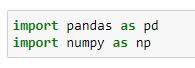
\includegraphics{Assets/Images/Pandas/import}
	\caption{Importing Pandas as pd}
	\label{fig:import}
\end{figure}

\noindent We would then load our dataset and import them as Pandas dataset.

\begin{figure}[ht]
	\centering
	\includegraphics[width=1.0\linewidth]{"Assets/Images/Pandas/read data"}
	\caption{Importing data}
	\label{fig:read-data}
\end{figure}

\noindent We can simply call the data by typing it's name (in this case \textit{drug}).
\begin{figure}[ht]
	\centering
	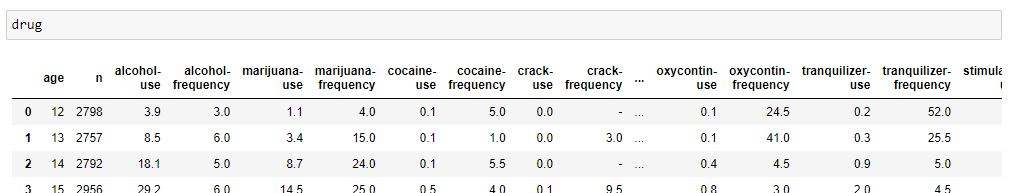
\includegraphics[width=1\linewidth]{Assets/Images/Pandas/drugs}
	\caption{Calling the data}
	\label{fig:drugs}
\end{figure}

\noindent If we only want to see the first few rows, we use the \textit{head} method. Which is 5 by default.

\begin{figure}[ht]
	\centering
	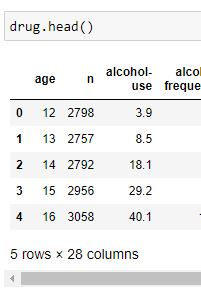
\includegraphics{Assets/Images/Pandas/head}
	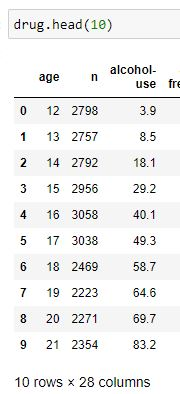
\includegraphics{Assets/Images/Pandas/head10}
	\caption{Using head method}
	\label{fig:head}
\end{figure}

\noindent Likewise, the \textit{tail} method for last few rows.

\begin{figure}[ht]
	\centering
	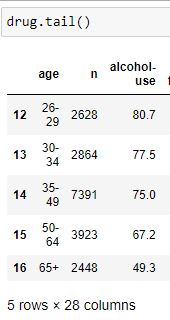
\includegraphics{Assets/Images/Pandas/tail}
	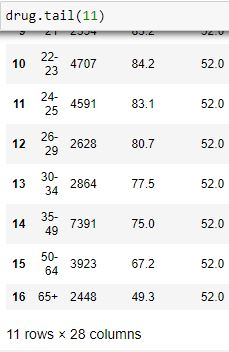
\includegraphics{Assets/Images/Pandas/tail11}
	\caption{Using tail method}
	\label{fig:tail}
\end{figure}

\newpage
\noindent The \textit{index} method is used to examine index which could be handy to detect duplicates

\begin{figure}[ht]
	\centering
	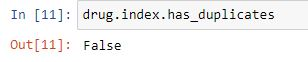
\includegraphics{Assets/Images/Pandas/index_duplicates}
	\caption{Using index method}
	\label{fig:index}
\end{figure}

\noindent We can use \textit{shape} method to examine the dimensions of our data.

\begin{figure}[ht]
	\centering
	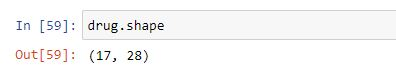
\includegraphics{Assets/Images/Pandas/shape}
	\caption{Using shape method}
	\label{fig:index}
\end{figure}
%\chapter{Exponential and Logarithmic Functions}
%\chapter{Limit and Differentiation}
%\chapter{Linear Algebra, Vector and Matrices}
%\chapter{Combinatorics and Probability}
\chapter{misc unorganized stuffs}
use logic table to understand confusion matrix better

\backmatter
\bibliography{citation} 
\bibliographystyle{ieeetr}
% bibliography, glossary and index would go here.

\end{document}